\documentclass[a4paper,11pt, twocolumn]{article}
\usepackage[margin=0.8in]{geometry}
\usepackage{xcolor}
\usepackage{graphicx} %package to manage images
\graphicspath{ {./images/} }
\usepackage{amsmath}

\title{A2-03 Communication Systems}
\author{Revision sheet}
\date{}

\usepackage{fancyhdr}
\pagestyle{fancy}
\fancyhead{} % clear all header fields
\renewcommand{\headrulewidth}{0pt} % no line in header area
\fancyfoot{} % clear all footer fields
\renewcommand{\footrulewidth}{0.4pt}
\fancyfoot[C]{\thepage} % page number in centre of the page
\fancyfoot[R]{\footnotesize Thomas Boxall \\ Images from WJEC E-Book} % right hand footer has author name on top line and images reference on bottom line
\fancyfoot[L]{\footnotesize A2-03 Communication Systems \\ Revision sheet} % left hand footer has title of document on top line and 'Revision Sheet' on bottom line


\begin{document}

\maketitle
\thispagestyle{fancy}

% CONTENTS OF THE REVISION SHEET HERE
\section{Introduction}
Shown below is the generic layout of a communication system.
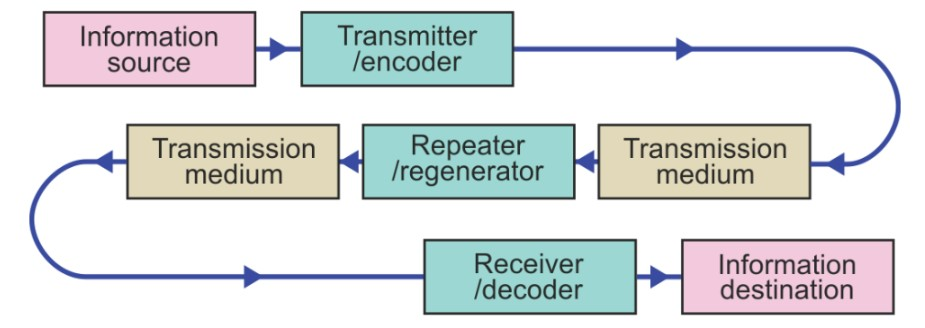
\includegraphics[width=0.45\textwidth]{genericSystemLayout.jpg}
Over a long distance, the signal quality degrades. To help overcome this, a repeater/ regenerator can be used to `boost' the signal. This could be an amplifier or another flaming basket on a stick.
\subsection{Bandwidth and Capacity}
Any transmission medium has \textit{available bandwidth} which it can transmit.
\subsubsection{Channel Bandwidth}
THe signals we want to transmit have a bandwidth, this is smaller than the available bandwidth therefore we can transmit several `channels' at once (using different carrier waves). We can calculate the number of channels ($N_{CH}$) using the following formula.\\
$\displaystyle N_{CH} = \frac{\mathrm{Available\ bandwidth}}{\mathrm{Channel\ bandwidth}}$

\section{Multiplexing}
THis is the process of allowing several independent users to share the same transmission medium.
\subsection{FDM}
\textit{Frequency Division Multiplexing} involves assigning non-overlapping frequency ranges to each signal. During transmission, each channel has a \textit{guard band} which prevents interference between bands. In the example shown below, there are three radio stations. have been allocated a bandwidth of $8KHz$, with a guard band of $2KHz$ between them. They are given carrier frequencies 80, 90 and 100 KHz respectively. Their frequency bands are shown below\\
Station 1 occupies a frequency band of ($80 \pm 4) KHz (=76 \Rightarrow 84) KHz$\\
Station 2 occupies a frequency band of ($90 \pm 4) KHz (=86 \Rightarrow 94) KHz$\\
Station 3 occupies a frequency band of ($100 \pm 4) KHz (=96 \Rightarrow 104) KHz$\\
The two different types of graphical representation are shown below.
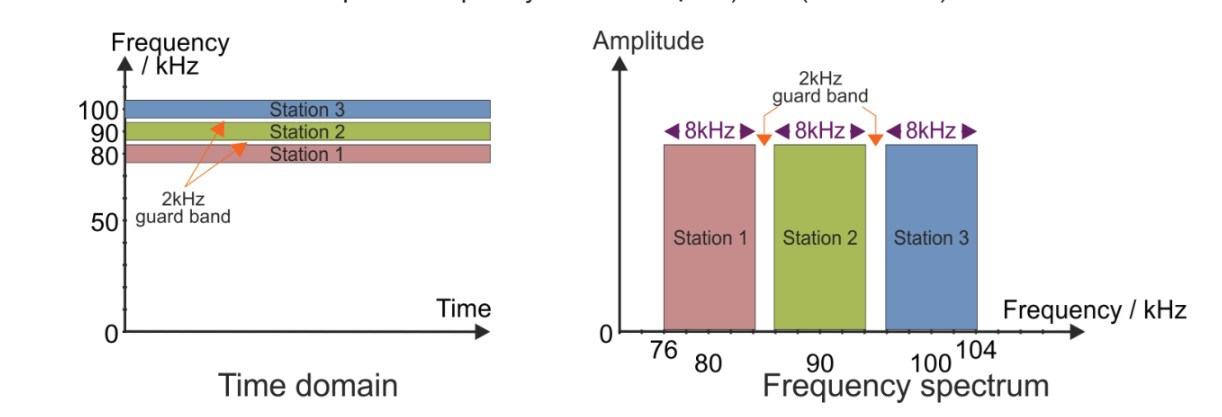
\includegraphics[width=0.45\textwidth]{fdm.jpg} 
\subsection{TDM}
\textit{Time Division Multiplexing} involves dividing the transmission time into timeslots of fixed length. These timeslots are cycled through, with each signal broadcasting part of its signal in its allocated time slot. During transmission, each signal has access to the full range of frequencies available to the channel.
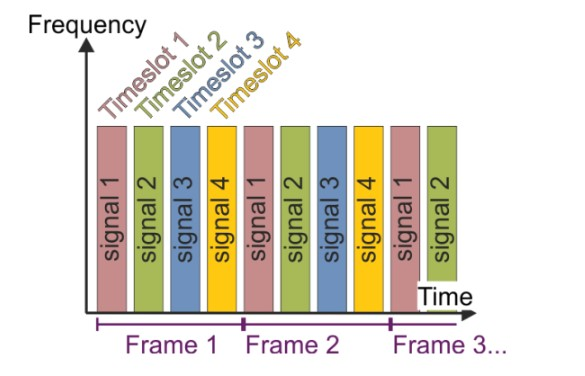
\includegraphics[width=0.45\textwidth]{tdm.jpg}

\section{Gain and Attenuation}
\subsection{Attenuation}
\textit{Attenuation} is the loss of signal strength over time, this means the amplitude of the signal diminishes. It can be thought of as gain which is less than 1. 
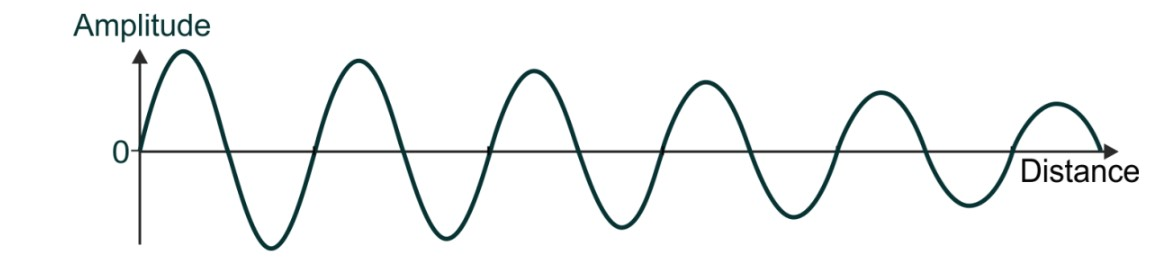
\includegraphics[width=0.45\textwidth]{attenuation.jpg}
\noindent Attenuation is measured in decibels per kilomiter ($dB/Km$)
\subsection{Gain}
\textit{Gain} is a measure of the ability of a sub-system to increase the voltage, current or power of a signal. 
\subsubsection{Voltage Gain}
$\displaystyle Gain = \frac{V_{out}}{V_{in}}$
\subsubsection{Power Gain}
In communication systems, the decibel (dB) is used to express the power gain of an amplifier or the power loss of a transmission medium.\\
$\displaystyle G_{dB} = 10 \log_{10}\frac{P_{OUT}}{P_{IN}}$\\
\textbf{Un-logging a log}\\
Logs and numbers surrounding them have the following relationships\\
$\displaystyle \log_{10}(a) = b$\\
$\displaystyle 10^b = a$
\subsubsection{Overall Gain}
In a system where there are two amplifiers connected in series, with the gains $G_1$ and $G_2$ respectively, the overall gain can be calculated using the following equation:\\
$G_1\times G_2 = G_{total}$\\
The overall gain in dB can be calculated using the following equation:\\
$G_1 + G_2 = G_{total}$

\section{Noise and Distortion}
\subsection{Distortion}
Distortion is where the signal is altered in a non-linear way (not just making it bigger/ smaller). One type of distortion is clipping distortion, shown below.
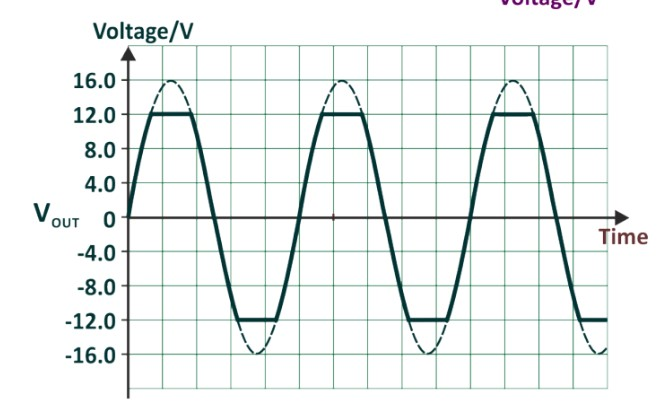
\includegraphics[width=0.45\textwidth]{clippingDistortion.jpg}
\subsection{Noise}
This is an external unwanted signal which is added to the signal. It can come from several sources: random noise, interference (from EM waves); cross talk (interference from other transmissions). 
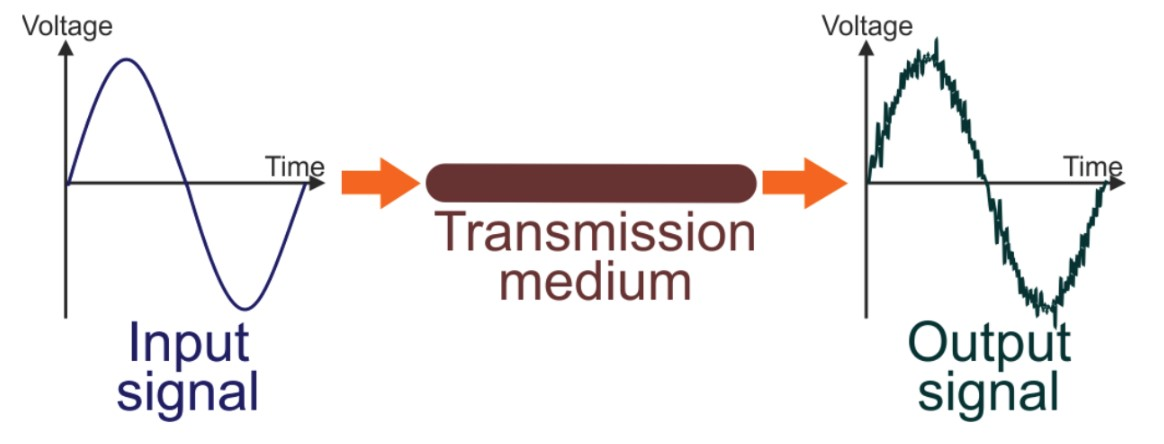
\includegraphics[width=0.45\textwidth]{noise.jpg}
Noise limits the distance of a transmission as signal amplitude decreases with distance while noise amplitude stays the same.
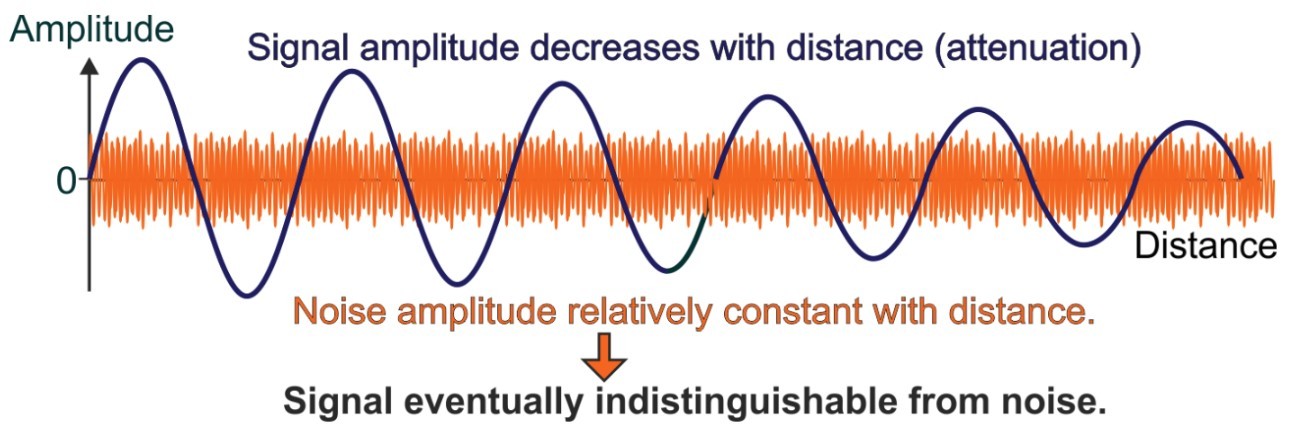
\includegraphics[width=0.45\textwidth]{noiseSignalAmplitude.jpg}

\section{Signal To Noise Ratio}
This is the ratio of signal amplitude to noise amplitude. SNR is calculated in decibels and the higher the value is, the better it is. If the SNR falls below 0dB, the signal power is equal to the noise power and the signal is unrecoverable. 
\begin{align*}
    SNR & = 20\log_{10}\left(\frac{P_S}{P_N}\right)\\
    & = 20 \log_{10}\left(\frac{V_S}{V_N}\right)
\end{align*}
\end{document}